
\section{Theorie}
\label{sec:Theorie}
\subsection{Relaxationsgleichung}
\subsubsection{Allgemeine Relaxationsgleichung}
Für ein aus dem Grundzustand ausgelenktes System, das nicht-oszillierend zu diesem zurückkehrt, gilt für die physikalische Größe $A$ zur Zeit $t$:
\begin{equation}
\frac{\mathrm{d}A}{\mathrm{d}t}=c\left[A(t)-A(\inf)\right]
\end{equation}
Die Integration von $0$ bis $t$
\[
\int_{A(0)}^{A(t)} \frac{\mathrm{d}A'}{A' - A(\inf)}=\int_0^tc\mathrm{d}t
\]
liefert 
\begin{equation}
A(t) = A(\inf) + \left[A(0)-A(\inf)\right]e^{ct}\text{.}
\end{equation}
Daraus folgt für $c$ die Bedingung $c<0$, da A beschränkt sein muss.
\subsubsection{Entladung eines Kondensators}
\label{sec:Entladung}
\begin{figure}
\centering
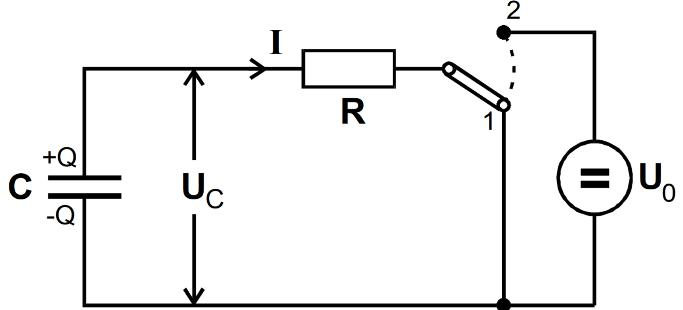
\includegraphics[scale=0.4]{content/images/theorie.jpg}
\caption{Schaltungen zur Auf- und Entladung eines Kondensators $C$ über den Widerstand $R$.\cite{V353}}
\label{fig:theorie}
\end{figure}
Für die in Abbildung \ref{fig:theorie} aufgebaute Schaltung gilt:
Zwischen den Platten eines Kondensators mit Kapazität $C$ Ladung $Q$  liegt die Spannung
\begin{equation}
U_.C=\frac{Q}{C}\label{eq:QC}
\end{equation}
an. Am Widerstand $R$ fließt außerdem der Strom
\begin{equation}
I = \frac{U_.C}{R}
\end{equation}
was zur Entladung führt.
Die Ladung der Kondensatorplatten ändert sich deshalb um
\begin{equation}
\mathrm{d}Q = - I\mathrm{d}t\label{eq:dQ}
\end{equation}
Daraus folgt für den zeitlichen Verlauf von $Q$ die Differentialgleichung
\begin{equation}
\frac{\mathrm{d}Q}{\mathrm{d}t} = - \frac{1}{RC}\cdot Q\text{.}
\label{eq:DGL}
\end{equation}
Mit der Bedingung, dass die Ladung für $t\rightarrow\inf$ 0 sein muss ergibt sich die Lösung:
\begin{equation}
Q(t) = Q(0)\cdot e^{\frac{-t}{RC}} \label{eq:Q1}
\end{equation}
$R\cdot C$ ist dabei die Zeitkonstante des Relaxationsvorgangs und bezeichnet die Zeitspanne, in der die Ladung sich um den Faktor $\frac{1}{e}$ ändert.
\subsubsection{Aufladung eines Kondensators}
\label{sec:Aufladung}
Bei der Aufladung gelten dieselben Voraussetzungen wie bei der Entladung. Nur die Randbedingung ändern sich hier, da $Q(0)=0$ und $Q(t\rightarrow\inf)=U_.{max}=CU_.0$ gelten, wobei $U_.0$ die Spannung des Generator ist.
Damit ergibt sich die Lösung
\begin{equation}
Q(t) = CU_.0\left(1-e^{\frac{-t}{RC}}\right) \label{eq:Q2}
\end{equation}
\subsubsection{Relaxation eines RC-Gliedes bei periodischer Auslenkung aus dem Grundzustand}
Liegt an einem $RC$-Schwingkreis eine Wechselspannung
\[
U(t)= U_.0\cdot cos(\omega t)
\]
an, führt das zu periodisch auftretenden Auf- und Entladevorgängen des Kondensators, wie sie in Abschnitt \ref{sec:Entladung} und \ref{sec:Aufladung} erläutert wurden.
Solange für die Kreisfrequenz gilt $\omega << \frac{1}{RC}$, ist $U_.C(t)$ nahezu identisch mit $U(t)$. Bei steigender Frequenz ist jedoch der Auf- und Entladevorgang zu langsam und es bildet sich bei gleichzeitig abnehmender Amplitude $A$ eine Phasenverschiebung $\phi$ zwischen Kondensator- und Generatorspannung aus.
Nach dem Kirchhoffschen Maschenregel gilt für einen RC-Stromkreis:
\begin{equation}
U(t)=U_.R(t)+U_.C(t)\label{eq:U1}
\end{equation}
und mit dem Ansatz für die Kondensatorspannung
\[
U_.C(t)= A(\omega)\cdot cos(\omega t + \phi (\omega))
\]
und mit Gleichung \eqref{eq:QC} und \eqref{eq:dQ}
\begin{equation}
U_.0\cdot cos(\omega t) = -A\omega RC\cdot sin(\omega t + \phi) + A(\omega)\cdot cos(\omega t + \phi)\text{.}\label{eq:U2}
\end{equation}
Da diese Gleichung für alle t gültig sein muss, kann die Frequenzabhängigkeit der Phase durch einsetzen von bestimmten Werten hergeleitet werden.
Einsetzen von $\omega t=\frac{\pi}{2}$ liefert:
\[
0 = -\omega RC\cdot sin\left(\frac{\pi}{2}+\phi\right)+ cos\left(\frac{\pi}{2}+\phi\right)
\]
Umformen und Ausnutzen der trigonometrischen Identitäten liefert
\begin{equation}
\phi (\omega)= arctan(-\omega RC)\label{eq:phi}
\end{equation}.
Um $\phi$aus den Messwerten zu bestimmen wird
\begin{equation}
\phi = \frac{a}{b}\cdot 360\label{eq:phi1}
\end{equation}
verwendet, wobei $a$ der Abstand der beiden Kurven an den Extremstellen und $b$ die Periodendauerdauer der Kondensatorspannung ist.
Desweiteren liefert das Einsetzen von $\omega t + phi = \frac{\pi}{2}$
\[
U_.0\cdot cos\left(\frac{\pi}{2}-\phi\right)= -A\omega RC
\]
und damit die Frequenzabhängigkeit der Amplitude $A$ der Kondensatorspannung
\begin{equation}
A(\omega)=-\frac{sin(\phi)}{\omega RC}\cdot U_.0\label{eq:A1}
\end{equation}
Mit Gleichung \eqref{eq:phi} und der Identität
\[
sin^2(\phi)+cos^2(\phi)=1
\]
folgt daraus
\begin{equation}
A(\omega)=\frac{U_.0}{\sqrt{1+\omega^2R^2C^2}}\label{eq:A2}
\end{equation}
\subsection{Integrator-Eigenschaft des RC-Glieds}
Aus den Gleichungen \eqref{eq:U1}, \eqref{eq:QC} und \eqref{eq:dQ}ergibt sich
\[
U(t)=RC\cdot\frac{\mathrm{d}U_.C}{\mathrm{d}t} + U_.C
\]
Für Frequenzen $\omega >> \frac{1}{RC}$ gilt $U_.C << U_.R$. Damit fällt der 2. Term weg und eine Integration liefert
\[
U_.C(t)=\frac{1}{RC}\int_0^tU(t')\mathrm{d}t\text{.}
\]
Das RC-Glied integriert also die ankommende Spannung $U(t)$